

\begin{enumerate}
\item Browse to the directory where you saved the setup file you downloaded. 
\item Double-click the file \bxcaption{setup.exe}. 
\item A welcome screen appears (\bxfigref{figWelcome}). Click \bxcaption{Next} to begin installation. 

\begin{center}
\begin{figure}[h]
  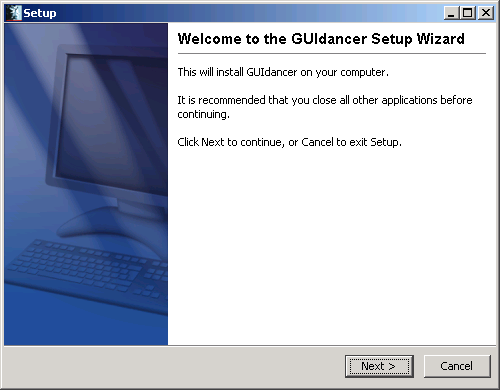
\includegraphics[width=10cm]{Windows/PS/welcome}
  \caption{Welcome Screen}
  \label{figWelcome}
\end{figure}
\end{center}


\item The license agreement will appear. Read it and accept it to continue.  
You can view and print this license later. It is saved in the installation directory and is called \bxname{license-agreement.txt}. 
\item At the next dialog, choose where to install the components. You can search or enter a directory or use the default. Click \bxcaption{Next}.
\item Choose the components to be installed.
You can install the \gdagent and the \ite{} on different machines if you want to.  If this is the case, carry out the installation for the other component (\gdagent or \ite{}) later. 

To be able to access the manual as a .pdf file, install the  documentation. Click \bxcaption{Next}.
 

\item Choose a start menu folder to create the shortcuts in. If you are installing as an administrator, there is a checkbox with the option to install the shortcuts for all users. To continue, click
\bxcaption{Next}. 
\item The selected components will  be installed.
\item Once the installation is finished, a dialog appears to confirm this (\bxfigref{complete}).

\begin{center}
\begin{figure}[h]
  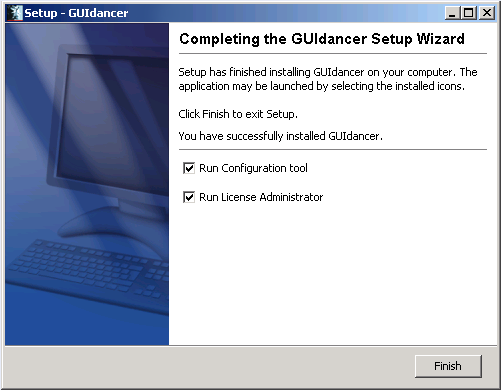
\includegraphics[width=10cm]{Windows/PS/complete}
  \caption{Installation complete}
  \label{complete}
\end{figure}
\end{center}


\item Click \bxcaption{Next} and then \bxcaption{Finish} to exit the installation wizard. 
\end{enumerate}




